\documentclass[a4paper]{article} 
\usepackage{geometry,fancyhdr,caption,subcaption,graphicx,psfrag,amsfonts,textcomp,mathtools,amsmath,hyperref} 

% settings courtesy of http://www.tjansson.dk/?p=419
\usepackage{listings}
\usepackage{color}
\usepackage{textcomp}
\definecolor{listinggray}{gray}{0.9}
\definecolor{lbcolor}{rgb}{0.9,0.9,0.9}
\lstset{
	backgroundcolor=\color{lbcolor},
	tabsize=4,
	rulecolor=,
	language=matlab,
        basicstyle=\scriptsize,
        upquote=true,
        aboveskip={1.5\baselineskip},
        columns=fixed,
        showstringspaces=false,
        extendedchars=true,
        breaklines=true,
        prebreak = \raisebox{0ex}[0ex][0ex]{\ensuremath{\hookleftarrow}},
        frame=single,
        showtabs=false,
        showspaces=false,
        showstringspaces=false,
        identifierstyle=\ttfamily,
        keywordstyle=\color[rgb]{0,0,1},
        commentstyle=\color[rgb]{0.133,0.545,0.133},
        stringstyle=\color[rgb]{0.627,0.126,0.941},
}

\title{Mandatory exercise 7 \\
Signal and Image Processing 2012} 
\author{Jens P. Raaby \\
\url{frn617@diku.dk}}

\begin{document} 
\maketitle

\section{Development of the compression method (WHAT I DID)}
\subsection{Encoding}
First I considered the steps that encoding would involve. Gonzalez \& Woods suggest the compression is first a mapping stage, then a quantizing stage, then a symbol coding stage. This latter stage is designed to simply remove the redundant information and minimise the storage required.

My first approach was to consider Huffman coding, as described in the lecture notes and Gonzalez \& Woods. I read about the more recent developments in image compression which use arithmetic coding instead. Both of these methods are designed to compress input data by removing


\subsection{Decoding}

\section{Reasons for choices (WHY I DID IT THAT WAY)}
\subsection{Types of redundancy, possible solutions, choices}
\begin{itemize}

    \item Coding redundancy


    \item Spatial redundancy


    \item Irrelevant information
\end{itemize}

\subsection{Options for storing parameters}

\section{Analysis of the results on the lena.bmp image}
\begin{itemize}

    \item reconstructed image

    \item SNR

    \item Comp ratio
\end{itemize}

\subsection{Properties of the Lena Image}


\section{Discussion of the results in general - potential improvements}

% \begin{figure}
%     
%         \centering
%         \begin{subfigure}[b]{0.4\textwidth}
%                 \centering
%                 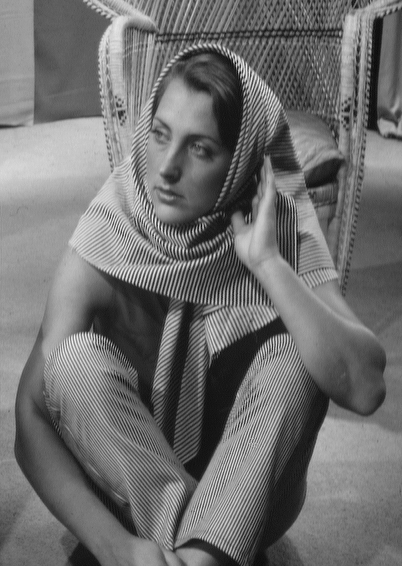
\includegraphics[width=\textwidth]{q4-orig.png}
%                 \caption{The Original IC.tif image}
%                 \label{fig4:orig}
%         \end{subfigure}
%         \begin{subfigure}[b]{0.4\textwidth}
%                 \centering
%                 \includegraphics[width=\textwidth]{q4-denoised.png}
%                 \caption{The denoised image}
%                 \label{fig4:denoise}
%         \end{subfigure}
%         
%         \caption{Decomposed signals}        
%         \label{fig4}
% \end{figure}

\clearpage
\% appendix 
% \section{Question 6.3 source} 
% \label{appendix-lst3} 
% \lstinputlisting{q63.m}
% \section{Question 6.4 source} 
% \label{appendix-lst4} 
% \lstinputlisting{q64.m}
\end{document} 
